\documentclass{article}
\usepackage[spanish]{babel}
\usepackage{lipsum}
\usepackage{natbib}
\usepackage{graphicx}
\usepackage{analysis_orax}
\usepackage{blindtext}
\usepackage{amsmath}
\usepackage{hyperref}
\usepackage{subcaption} 
\usepackage{float}
\usepackage{listings}
\usepackage{pxfonts}
\usepackage{svg}
\usepackage{pgfplots}
\pgfplotsset{compat=1.11}
\usepackage{enumitem}
\usepackage{tikz}
\usetikzlibrary{shadows}

\newcommand*{\MyShadow}{\tikz \draw [baseline, fill=blue,draw=blue,circular drop shadow] circle (2pt);}
\newcommand*{\MyBall}{\tikz \draw [baseline, ball color=red, draw=red] circle (2pt);}

\definecolor{mGreen}{rgb}{0,0.6,0}
\definecolor{mGray}{rgb}{0.5,0.5,0.5}
\definecolor{mPurple}{rgb}{0.58,0,0.82}
\definecolor{backgroundColour}{rgb}{0.95,0.95,0.92}

\lstdefinestyle{CStyle}{
    backgroundcolor=\color{white},   
    commentstyle=\bfseries \color{darkgray},
    keywordstyle=\color{LightBlue}\bfseries,
    numberstyle=\tiny\color{white},
    stringstyle=\color{mPurple},
    basicstyle=\footnotesize \color{mPurple},
    breakatwhitespace=false,         
    breaklines=true,                 
    captionpos=b,            
    keepspaces=true,                 
    numbers=left,                    
    numbersep=5pt,                  
    showspaces=false,                
    showstringspaces=false,
    showtabs=false,                  
    tabsize=2,
    language=C
}





\title{\bigskip \bigskip \bigskip \bigskip \vspace{-15mm}\fontsize{35pt}{35pt}\selectfont\textbf{{Trabajo práctico Nº II - OpenMP \\}}
\bigskip \bigskip \fontsize{18pt}{10pt}\selectfont\textbf{\textcolor{teal}{CÁTEDRA DE SISTEMAS OPERATIVOS II}}\bigskip\bigskip \bigskip\bigskip \bigskip}\bigskip\bigskip \bigskip\bigskip \bigskip % Article title
\author{
\large
{
\textsc{Casabella Martin, 39694763 }}\\[2mm]
  martin.casabella@alumnos.unc.edu.ar\\[2mm]
%\thanks{A thank you or further information}\\ % Your name
%\normalsize \href{mailto:marco.torres.810@gmail.com}{marco.torres.810@gmail.com}\\[2mm] % Your email address
\bigskip\bigskip \bigskip \bigskip\bigskip \bigskip
}

\date{\Huge\today}

%------------------Document----------------------------

\begin{document}
\maketitle
\clearpage

%-------------------------TitlePage------------------------
%\begin{titlepage}
%\end{titlepage}
%----------------------------------------------------------------------------------------
%       TITLE SECTION
%----------------------------------------------------------------------------------------

\renewcommand{\figurename}{\textbf{\textcolor{Orange}{Figura}}}
\renewcommand\thefigure{\textbf{\textcolor{Orange}{\arabic{figure}}}}

%-------------------------Content------------------------
\tableofcontents

\clearpage


\section{Introducción}
Los niveles de integración electrónica han permitido la generación de procesadores de arquitecturas multiprocesos, multicore y ahora many integrated core
(MIC). Este avance hace necesario que los programadores cuenten con un profundo conocimiento del hardware sobre el que se ejecutan sus programas, y que
dichos programas ya no pueden ser monoproceso.\\

Entre las técnicas y estándares mas utilizados para sistemas de memoria compartida y memoria distribuida, se encuentra OpenMP y MPI respectivamente.
\subsection{OpenMP}
OpenMP es una interfaz de programación de aplicaciones (API) para la programación multiproceso de memoria compartida en múltiples plataformas. \\

Permite añadir concurrencia a los programas escritos en C, C++ y Fortran sobre la base del modelo de ejecución fork-join. Está disponible en muchas arquitecturas, incluidas las plataformas de Unix y de Microsoft Windows. Se compone de un conjunto de directivas de compilador, rutinas de biblioteca, y variables de entorno que influyen el comportamiento en tiempo de ejecución.\\
\subsection{Propósito}
En el trabajo se pretende desarrollar la solucion de un problema de una convolucion bidimensional que presenta cierto tipo  de paralelismo.
Primero debe proponerse una solcion procedural, y luego una que explote el paralelismo inherente del problema.\\

Para ello, deben madurarse y entenderse los conceptos del funcionamiento del estándar OpenMP, sus aplicaciones, ventajas y desventajas.\\

\subsection{Ámbito del sistema}
Se requiere realizar una convolución bidimensional a partir de los datos extraídos de un satélite, que se reciben en forma de archivo con el formato \textit{.nc} del estandar \textit{netCDF4}. La convolución debe ser monocore y multicore, de tal manera que se puedan comparar los resultados.

\subsection{Definiciones, acrónimos y abreviaturas}
\subsection{netCDF}
Son librerías permiten compartir información tecnológica y científica en un formato auto definido, independiente de la arquitectura del sistema y también
definen un formato de datos que se transformo en estándar abierto. La librería tiene versiones en Fortran, Python, Java y C, siendo estas ultimas las que vamos
a utilizar en este trabajo.\\
\subsubsection{Datos netCDF}
El netCDF (formulario de datos comunes en red) es un formato de archivo destinado a almacenar datos científicos multidimensionales (variables) como la temperatura, la humedad, la presión, la velocidad del viento y la dirección. Cada una de estas variables se puede mostrar mediante una dimensión (por ejemplo, tiempo) en ArcGIS creando una vista de tabla o de capa a partir del archivo netCDF.
\subsection{Convolucion bidimensional y filtro}
Las imágenes digitales son consideradas como señales discretas bidimensionales, las cuales son procesadas por sistemas discretos o filtros. \\
La operación fundamental en lo que abarca el procesamiento de imágenes, es la convolución en dos dimensiones, entre la imagen (o señal de entrada) con el filtro mencionado, denominado kernel.\\
  \begin{figure}[H]
    \centering
      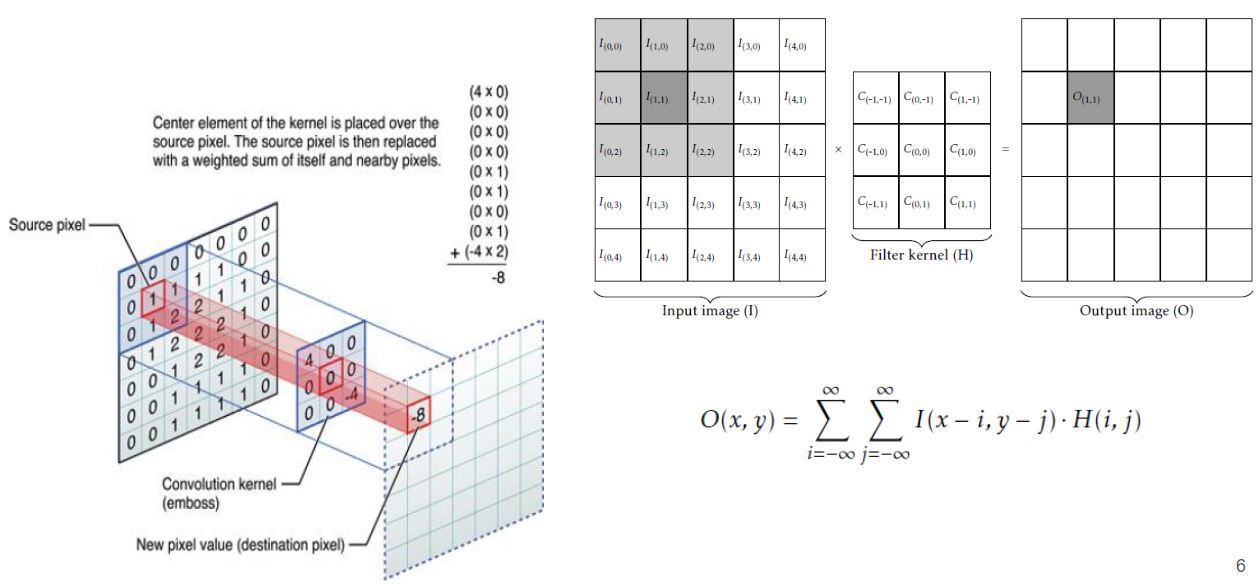
\includegraphics[width=0.65\textwidth]{figures/CONV.jpg}
       \centering
       \caption{\textbf{\textcolor{Orange}{Operación de convolucion 2D}}}\label{fig:1}
    \end{figure}
    
Al variar los coeficientes del filtro discreto (o kernel) empleado, se producen diferentes efectos en la imagen procesada:
  \begin{figure}[H]
    \centering
      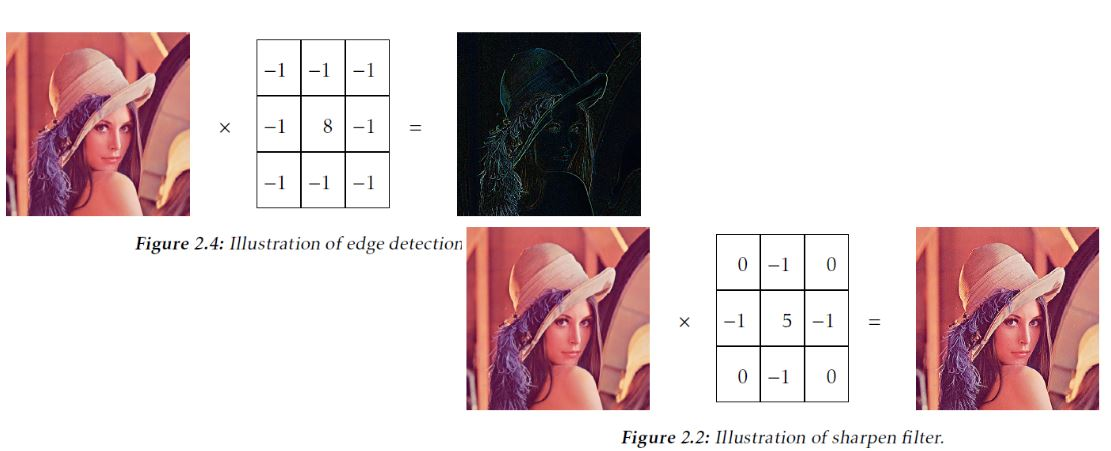
\includegraphics[width=0.65\textwidth]{figures/CONV2.jpg}
       \centering
       \caption{\textbf{\textcolor{Orange}{Influencia del filtro utilizado}}}\label{fig:1}
    \end{figure}
\subsubsection{Bordes}
Cuando la ventana de convolución se centra en el primer píxel de una imagen en (0,0), la máscara del kernel sobresale de la imagen en el borde superior y en el izquierdo.\\
Hay mas de una manera de resolver el tema. Se opto por la solución en que el pixel que va a ser procesado tiene que tener una ventana de convolución dentro de de los límites de la imagen, de tal manera que los pixeles de los bordes no se procesarán.\\
\clearpage
\subsection{Descripción general del documento}
Este documento esta organizado en 6 secciones principales:
\begin{enumerate}
\item Describe las generalidades del documento y del proyecto
\item Describe la perspectiva del producto, funciones del mismo, características de usuario y restricciones
\item Referencia a los requerimientos del producto, interfaces y casos de uso. Incluye diagramas y gráficos que facilitan su entendimiento
\item Abarca un diseño de la solución
\item La última parte incluye la implementación de la solución y resultados
\item Por último, se encuentran las conclusiones
\end{enumerate}
\section{Descripción general}
En la siguiente sección se presenta una breve descripción de los requisitos del sistema, sin entrar en detalle se explica las principales características del software.\\
\subsection{Perspectiva del Producto}
Como objetivo esta el diseño e implementación de un software desarrollado en lenguaje C. El componente principal es un archivo \textit{.nc} que alberga los datos de una imagen satelital que consiste en una matriz de tipo de dato \textit{float}. Al mismo se lo debe importar y leer, para así procesarlo en la convolución y guardarlos en un nuevo archivo. \\

Se generan archivos de salida tanto binarios, como en formato \textit{.nc}, y se desarrollo un script en Python 2 que se encarga de leer dichos archivos y generar las correspondientes imagenes en formatos \textit{png} y \textit{svg}.\\
\subsection{Funciones del Producto}
 El producto no posee una interfaz interactiva con el usuario, si no que solo se ejecuta lee el archivo, realiza la convolución y genera los correspondientes archivos de salida.\\
\begin{itemize}
\item \textbf{Lectura}:Lectura del archivo .nc y almacenamiento en memoria de los datos extraídos
\item \textbf{Convolución}: Calculo de la convolución con 3 implementaciones diferentes (procedural, y dos formas donde se explota el paralelismo)
\item \textbf{Escritura de salida}: Almacenamiento de la imagen filtrada resultante como archivos binarios (procedural, primer version paralela), y archivo \textit{.nc} (segunda versión paralela
\end{itemize}
\subsection{Características de los Usuarios}
El producto se destina a usuarios con los conocimientos básicos de manejo de sistemas operativos Linux. Se incluyeron un script para la versión local, y otro diferente para el cluster, que automatizan la compilación, ejecución y copia de archivos de salida.\\
\subsection{Restricciones, Suposiciones y Dependencias}
Se necesitara de un compilador GCC, junto con las librerías netCDF, netlib, glibc y lib instaladas.\\
En caso que se desee, se puede compilar a mano y cambiar los directorios. Caso contrario, los scripts mencionados incluyen todas las etapas. 
\section{Requisitos específicos}
Se detallan a continuación los requisitos específicos del sistema, especificados por el cliente.
\subsection{Interfaces externas}
Para el desarrollo del software se utiliza utiliza GNU/Linux, herramientas de compilación y librerías en su última versión estable, específicamente las versiones que cumplen los criterios son las rolling release como ArchLinux, Antergos, Manjaro y derivados:
\begin{itemize}
\item Kernel >= 5.0.7  ( 5.0.7-1-ARCH aarch64 GNU/Linux)
\item GCC >= version 8.2 
\item GLibC >= 2.26
\item Make >= 4.2.1
\item libnet >= 1.1.6-3 
\item netcdf  >= 4.7
\item python >= 2.7.16-1
\item python2-netcdf4  >= 1.5.1.2
\item python2-matplotlib  >= 2.2.4
\end{itemize}
\subsection{Requisitos funcionales}
El sistema no es interactivo. Debe ejecutarse, escribir resultados, terminar y salir del mismo. El archivo sera ejecutado de la forma conveniente para el usuario, por consola con
los respectivos permisos necesarios, o por interfaz gráfica con los mismos permisos.\\

\subsection{Requisitos de rendimiento}
El sistema debe ser capaz de correr en un SoC o una computadora personal (x86/AMD64), con al menos 4gb de ram y 8gb de espacio libre, un procesador con una frecuencia de 1GHz contando que solo compite en los recursos con los procesos del sistema operativo base. El sistema operativo base puede ser GNU/Linux o derivados de BSD.\\
\subsection{Requisitos de diseño}
Las restricciones incluyen el desarrollo de ambas soluciones en lenguaje C, utilizando la libreria OpenMP.\\
\subsection{Atributos del sistema}
\begin{itemize}
\item Capacidad de la utilización de sistemas operativos tipo UNIX, con escasos recursos necesarios
\item Escalabilidad en cuanto al grado de paralelismo
\end{itemize}

\section{Diseño de la solución}
La solución está documentada en el repositorio del proyecto.
Se trabajo con tipo de dato \textit{float}, y se generaron tres tipos de operación de filtrado de bordes (convolucion 2D):\\
\begin{enumerate}
\item \textbf{Procedural:} Forma típica de realizar esta operación: realiza la acumulación de los productos de los coeficientes del kernel con la sección correspondiente de la imagen antes de desplazarse horizontal o verticalmente para generar un nuevo pixel de salida. 
\item \textbf{Paralela v1 (parallel collapse):} Algoritmo anterior pero paralelizado. Ya que consta de cuatro bucles anidados, se aplico el pragma \textit{parallel collapse}.La caracteristica de esta directiva para paralelizar el bucle es que colapsa los bucles formando un solo bucle largo (sea primer bucle el limite \textit{N} y el limite del otro \textit{M}) formando un solo bucle de \textit{N} $x$ \textit{M}, que luego paraleliza.\\
\item \textbf{Paralela v2 (parallel for):} Esta solución esta basada en el pragma \textit{parallel for} donde puede setearse el numero de hilos a utilizar según los recursos que se dispongan. Básicamente se divide el bucle para que cada thread del conjunto creado, maneje una porción diferente de dos bucles anidados, que se encargan de ir moviendo el kernel a través de la imagen (horizontal o verticalmente, ya que en este caso es una matriz con la misma cantidad de filas que de columnas).
\end{enumerate}
\section{Implementación y resultados}
En cuanto a medida de tiempo, se utilizo la función  \textit{omp\_get\_wtime()} brindada por la librería. Esta función devuelve un valor de tiempo de doble precisión, que equivale al numero de segundos del clock de tiempo real del sistema operativo. Se garantiza que este valor no cambia durante la ejecución del programa.\\

Iniciando este clock previo a llamar a la función, y luego al volver (habiendo terminado la operación de convolución) restando el correspondiente tiempo de inicio, se puede obtener
el tiempo que demoro la operación en si. \\

Se ejecuto 50 veces el programa, variando el numero de threads, en un rango de 2 a 24  para la computadora local.\\

En cuanto al cluster, también se ejecuto 50 veces el programa, variando el numero de threads, hasta llegar a 32 threads instanciados. Esto se debe a las prestaciones
que ofrecía el mismo. \\

\clearpage
Se ejecuto en una computadora local, con las siguientes prestaciones en cuanto al procesador:
 \begin{figure}[H]
    \centering
      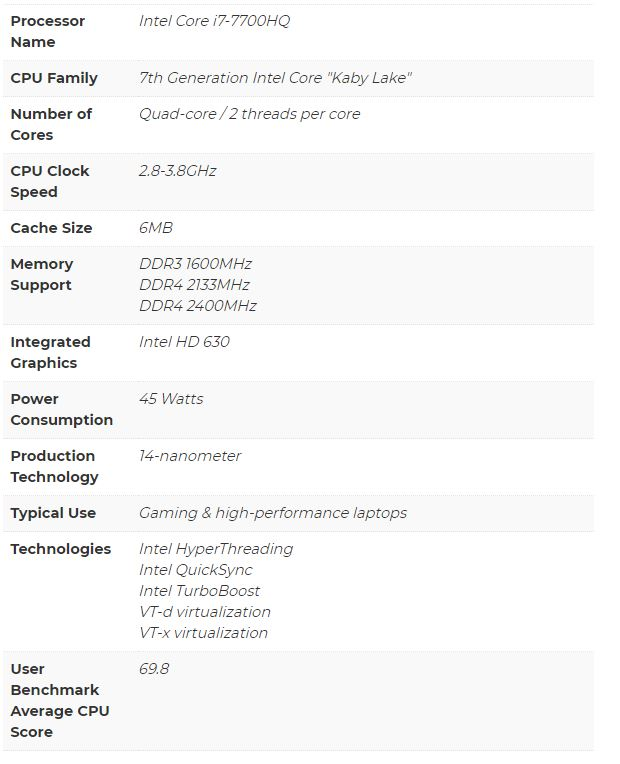
\includegraphics[width=0.50\textwidth]{figures/MICRO1.jpg}
       \centering
       \caption{\textbf{\textcolor{Orange}{Prestaciones del procesador de la computadora local}}}
    \end{figure}

En cuanto al cluster, el mismo dispone de Posee dos pastillas Intel Xeon Gold 6130 con 64Gb de ram (4 canales):
 \begin{figure}[H]
    \centering
      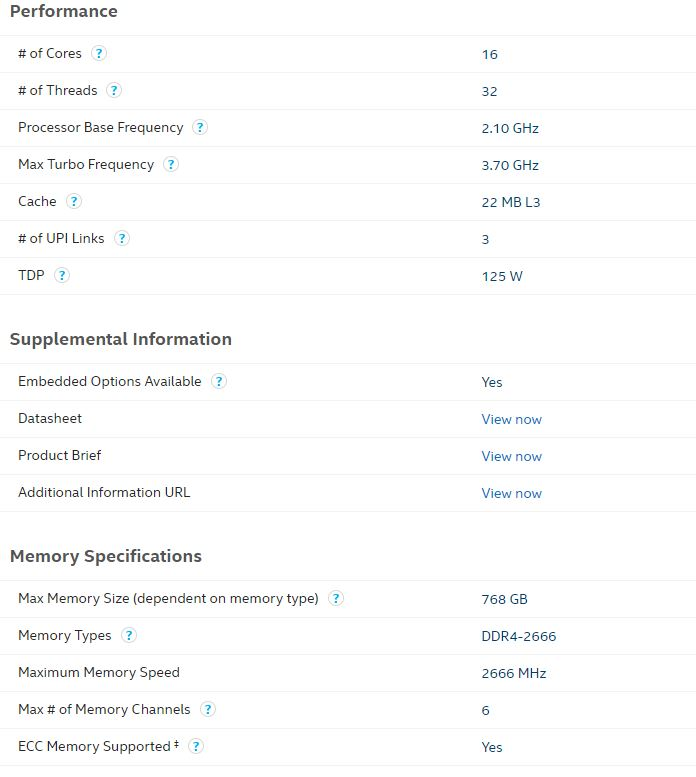
\includegraphics[width=0.50\textwidth]{figures/MICRO2.jpg}
       \centering
       \caption{\textbf{\textcolor{Orange}{Prestaciones del procesador del cluster}}}
    \end{figure}

\subsection{Profiling}
\subsubsection{Valgrind/Callgrind}
Valgrind es un conjunto de herramientas libres que ayuda en la depuración de problemas de memoria y rendimiento de programas. La herramienta más usada es Memcheck. Memcheck introduce código de instrumentación en el programa a depurar, lo que le permite realizar un seguimiento del uso de la memoria y detectar problemas. \\

La opción –leak-check activa el “memory leak detector”. El programa se ejecutará con una velocidad inferior a la normal(en un orden de 20-30\%), y usará una cantidad de memoria mayor. Memcheck emitirá mensajes sobre las “fisuras” y resto de errores de memoria que detecte.\\

Aspectos a tener en cuenta:
\begin{itemize}
\item En cada mensaje de error aparece mucha información. Sería conveniente leerlos con detalle.
\item El número entre ==number== es el identificador de proceso (PID). Normalmente carece de importancia.
\item La primera línea ("Invalid write...") indica cual es el error. Aquí indica que el programa escribió en alguna zona de memoria en la que no tendría que haberlo hecho debido a un “heap block overrun”.
\item A continuación de la primera línea se puede ver una traza de la pila que te dice donde ocurrió el problema. Las trazas de pila pueden tener un tamaño considerable, y ser confusas, especialmente si estás usando el C++ STL. Puede ser útil leerla desde abajo hacia arriba. Si la traza de la pila no es lo suficientemente grande, usa una opción –num-callers mayor.
\item Las direcciones (ej. 0x804838F) no son importantes normalmente, pero ocasionalmente son cruciales para seguir la traza de los errores más extraños.
\item Algunos mensajes de error tienen un segundo componente que describe las direcciones de memoria involucradas
\end{itemize}

Haciendo uso de memcheck, se obtuvo:
 \begin{figure}[H]
    \centering
      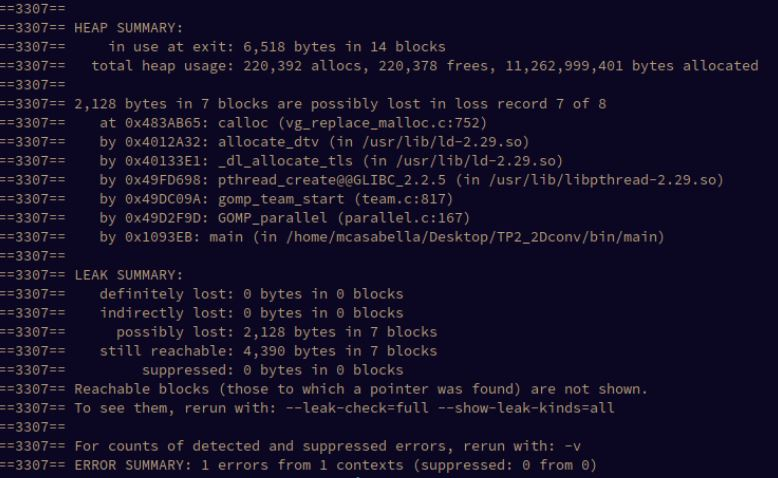
\includegraphics[width=0.90\textwidth]{figures/MEMORYLEAK.jpg}
       \centering
       \caption{\textbf{\textcolor{Orange}{Chequeo de perdida de memoria ('memory leak')}}}
    \end{figure}
\clearpage

A su vez, otra herramienta es \textit{Callgrind}, la cual genera un informe detallado sobre cada rutina del programa, entregando el porcentaje de tiempo que éstas ocupan
respecto al tiempo total de ejecución, el número de veces que éstas son ejecutadas y con cuáles otras rutinas interaccionan.\\

Callgrind corre en el framework Valgrind, y cuando se utiliza para hacer profiling para cierta aplicación, la aplicacion se transforma en un lenguaje intermedio y luego corre en un procesador virtual emulado por Valgrind. Esto tiene un gran overhead de tiempo de ejecución (de 10 a 50 veces mas lento), pero la precisión del profiling es realmente buena. \\

Adicionalmente, para este análisis se utiliza la herramienta de visualización denominada KCachegrind  la cual permite obtener una mejor visión general de la información generada por Cachegrind y Callgrind.  KCachegrind transforma la información en tablas y grafos para su fácil interpretación:

\begin{figure}[H]
  \begin{subfigure}[b]{0.50\textwidth}
    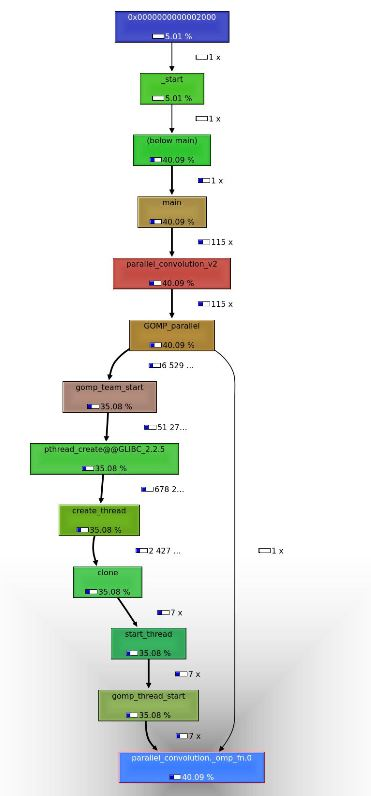
\includegraphics[width=\textwidth]{figures/parallel1.jpg}
     \caption{\textbf{\textcolor{Orange}{Grafo de la función de convolución paralela v1}}}
    \label{fig:41}
  \end{subfigure}
  %
  \begin{subfigure}[b]{0.50\textwidth}
    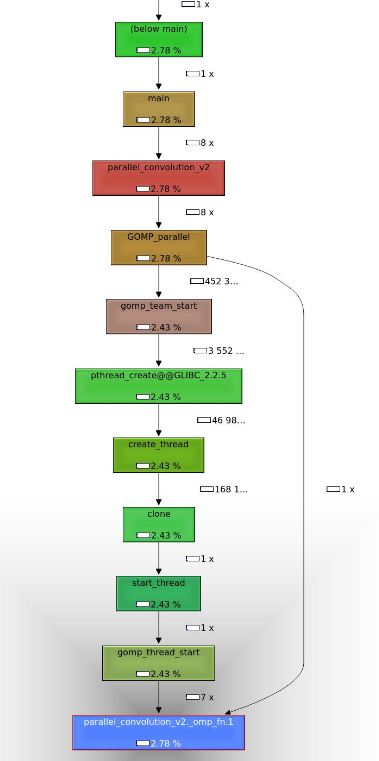
\includegraphics[width=\textwidth]{figures/parallel2.jpg}
     \caption{\textbf{\textcolor{Orange}{Grafo de la función de convolución paralela v1}}}
    \label{fig:42}
  \end{subfigure}
\end{figure}

\begin{figure}[H]
  \begin{subfigure}[b]{0.44\textwidth}
    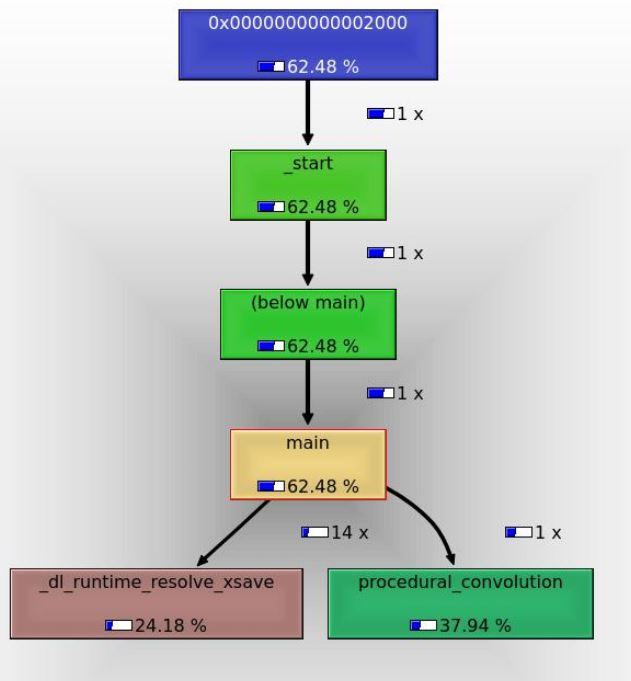
\includegraphics[width=\textwidth]{figures/main.jpg}
     \caption{\textbf{\textcolor{Orange}{Grafo de la función principal del programa (main) que llama a las demás}}}
  \end{subfigure}
  %
  \begin{subfigure}[b]{0.43\textwidth}
    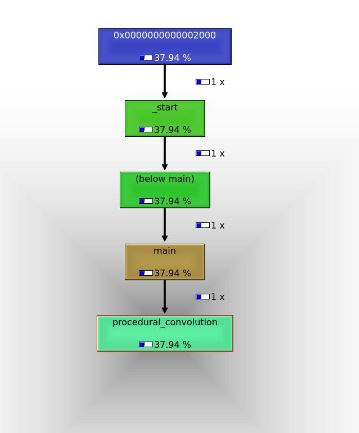
\includegraphics[width=\textwidth]{figures/profprocedural.jpg}
     \caption{\textbf{\textcolor{Orange}{Grafo de la función de convolución procedural}}}
    \label{fig:42}
  \end{subfigure}
\end{figure}

\begin{figure}[H]
    \centering
      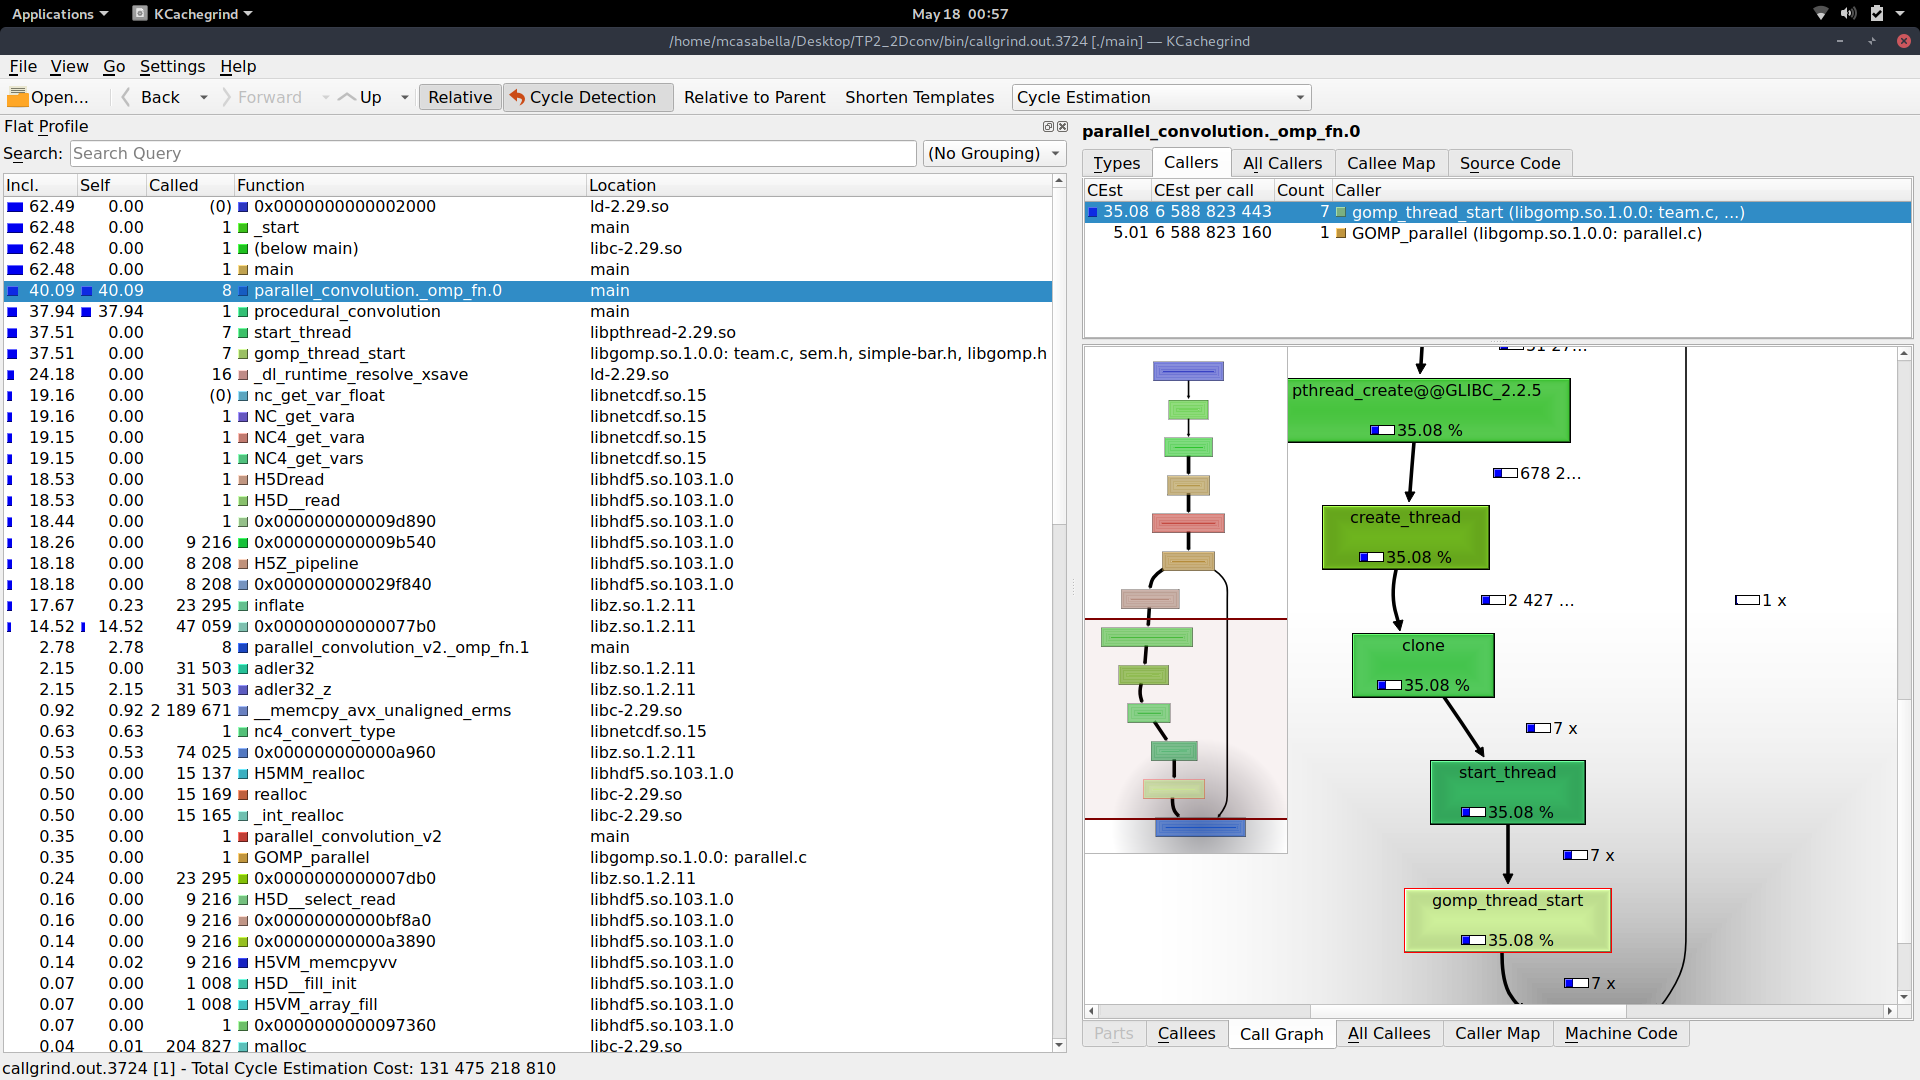
\includegraphics[width=1.0\textwidth]{figures/interfaz.png}
       \centering
       \caption{\textbf{\textcolor{Orange}{Apertura del archivo generado por la ejecucion de Callgrind, mediante el software KCachegrind}}}
    \end{figure}
\clearpage
\subsubsection{Perf}
Perf es una herramienta de análisis de performance que se accede como cualquier comando linux y provee de una serie de subcomandos.\\

Perf puede obtener varios datos desde aquellos que son parte del sistema o bien procesos realizados por el usuario, proporciona contadores de hardware, puntos de rastreo (tracepoints), contadores de perfomance de software, pruebas dinámicas, entre otros. La mayoría de la funcionalidad de Perf se encuentra integrada desde el kernel.\\

Es posible usar el comando \textit{perf stat n} y ejecutar la misma carga de trabajo de prueba \textit{n} veces , y obtener por cada cuenta, la desviación estándar de la media.
\begin{figure}[H]
    \centering
      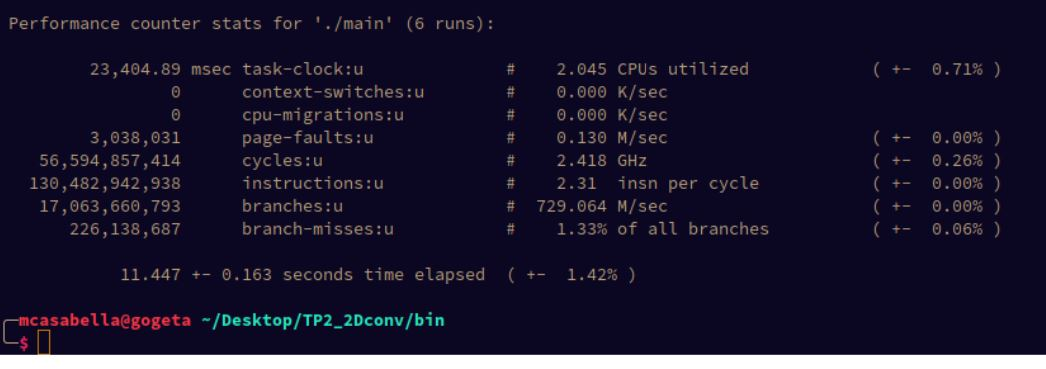
\includegraphics[width=1.0\textwidth]{figures/perf.jpg}
       \centering
       \caption{\textbf{\textcolor{Orange}{Profiling con perf para 6 ejecuciones con un número fijo de threads (8)}}}
    \end{figure}

\subsection{Imágenes procesadas}
\begin{figure}[H]
    \centering
      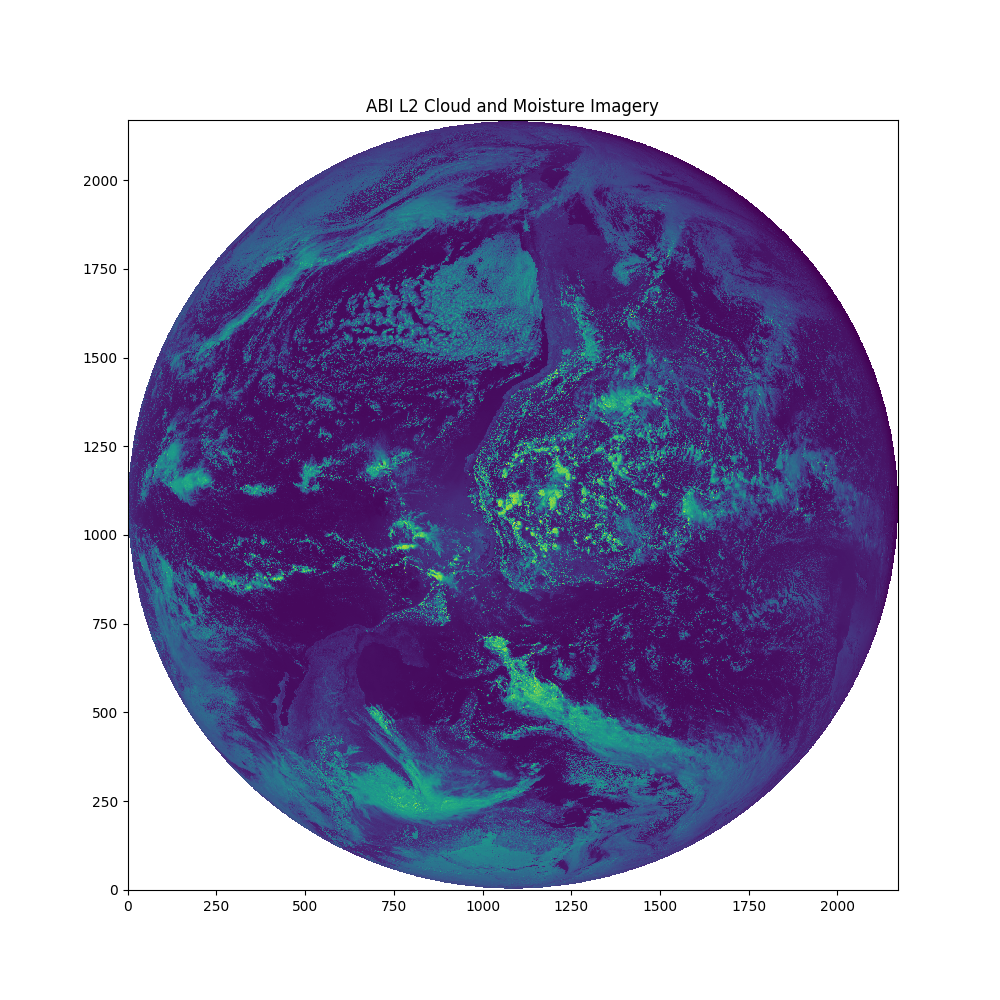
\includegraphics[width=1.0\textwidth]{figures/imagen1.png}
       \centering
       \caption{\textbf{\textcolor{Orange}{Imagen original ploteada desde Python, desde archivo .nc}}}
    \end{figure}
    
    Respecto a la convolucion procedural, su salida se almacena en un archivo binario. \\
    Se realizo lo mismo con los datos del archivo .nc para generar un binario con la imagen original.\\
    
     Luego, utlizando Python, se graficron las mismas donde se variar el rango de valores de cada pixel utilizando la \textit{matplotlib.pyplot.imshow}.\\
    
    \begin{figure}[H]
    \centering
      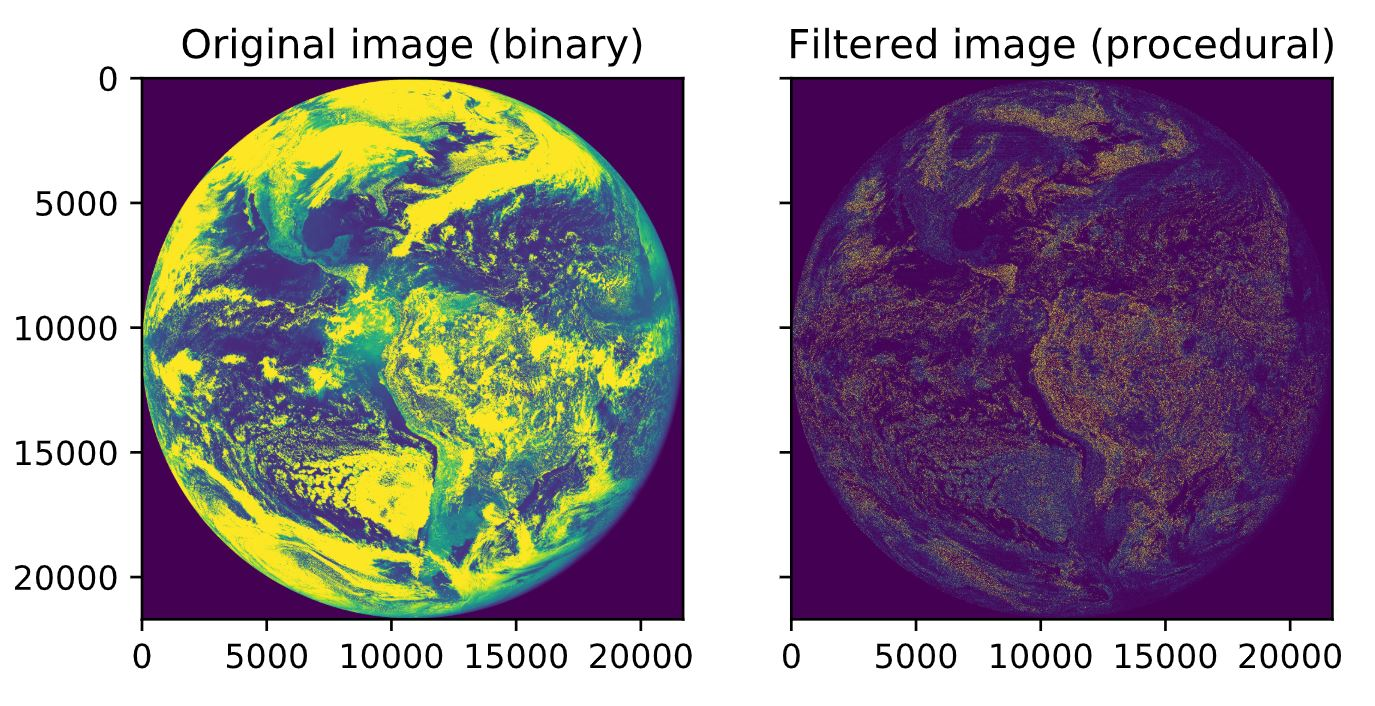
\includegraphics[width=1.0\textwidth]{figures/procedural.jpg}
       \centering
       \caption{\textbf{\textcolor{Orange}{Imagenes binarias ploteadas, sin especificar mapeo de colores}}}
    \end{figure}

    \begin{figure}[H]
    \centering
      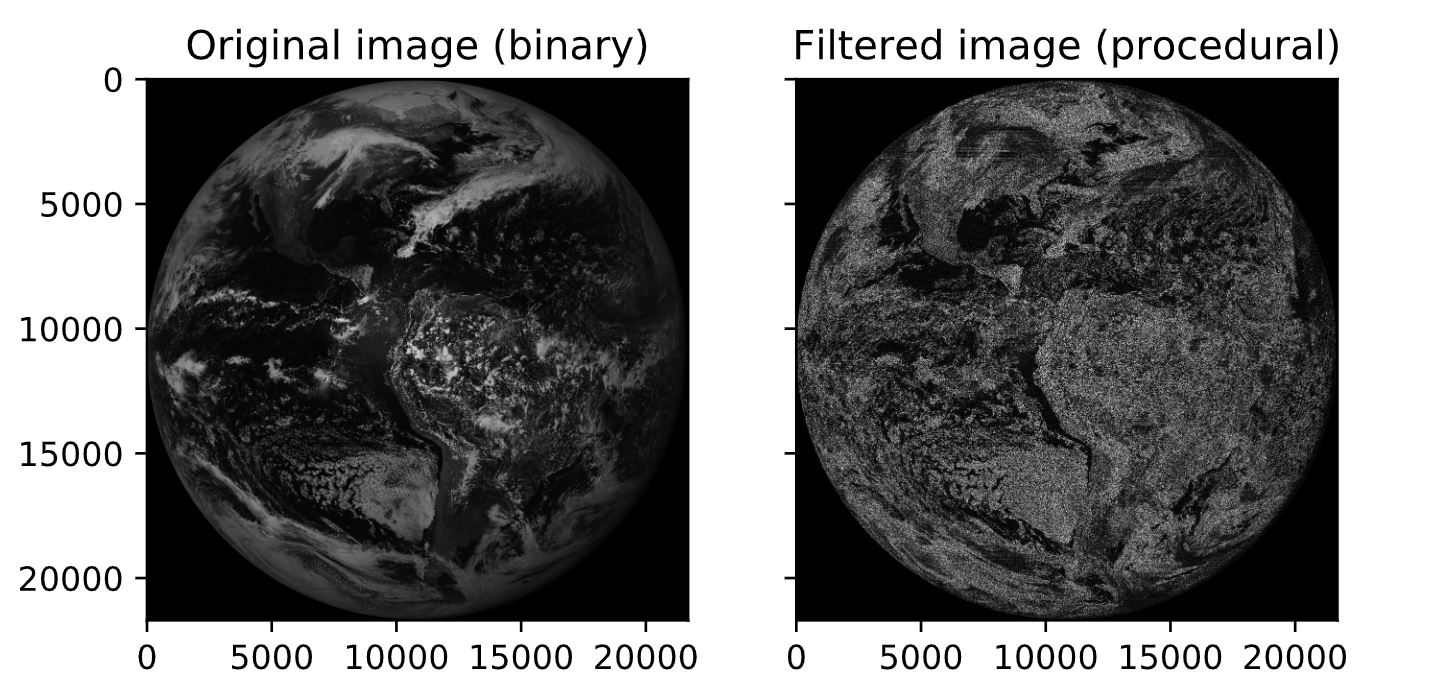
\includegraphics[width=1.0\textwidth]{figures/procedural_grey.jpg}
       \centering
       \caption{\textbf{\textcolor{Orange}{Imagenes en escala de grises}}}
    \end{figure}

    \begin{figure}[H]
    \centering
      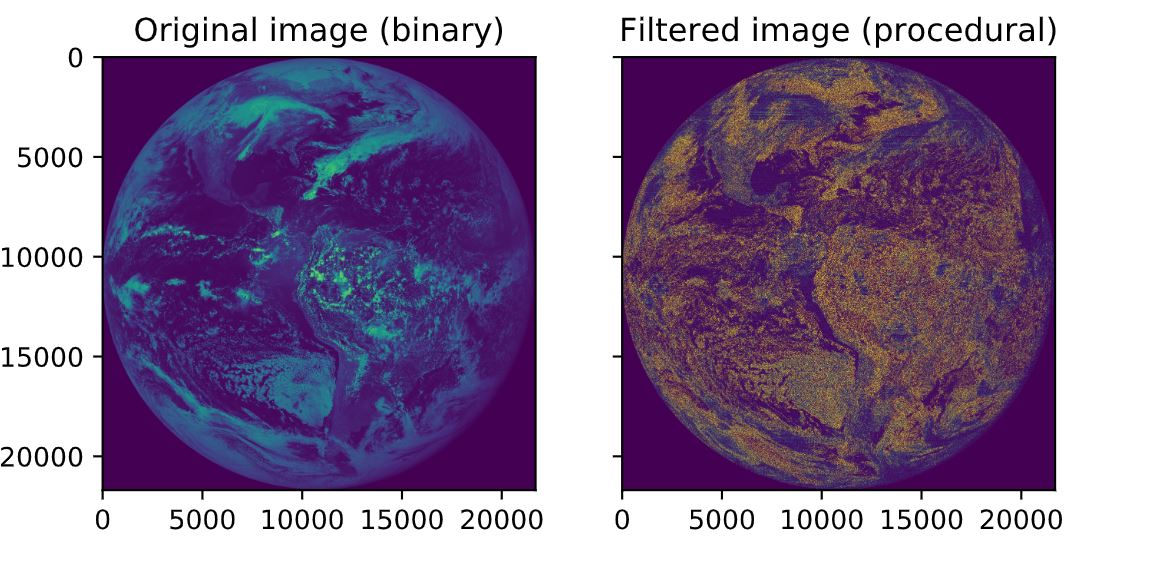
\includegraphics[width=1.0\textwidth]{figures/procedural_change_sat.jpg}
       \centering
       \caption{\textbf{\textcolor{Orange}{Imagenes variando rango de valores (min-max)}}}
    \end{figure}
    
    Se busco mostrar que la imagen filtrada tiene calidad aceptable, y que el cambio en el rango de valores es lo que afecta la escala de colores y tonalidades. Fijemos la misma escala, y veamos la imagen obtenida con la primer forma de convolucion paralela:\\
        
    \begin{figure}[H]
    \centering
      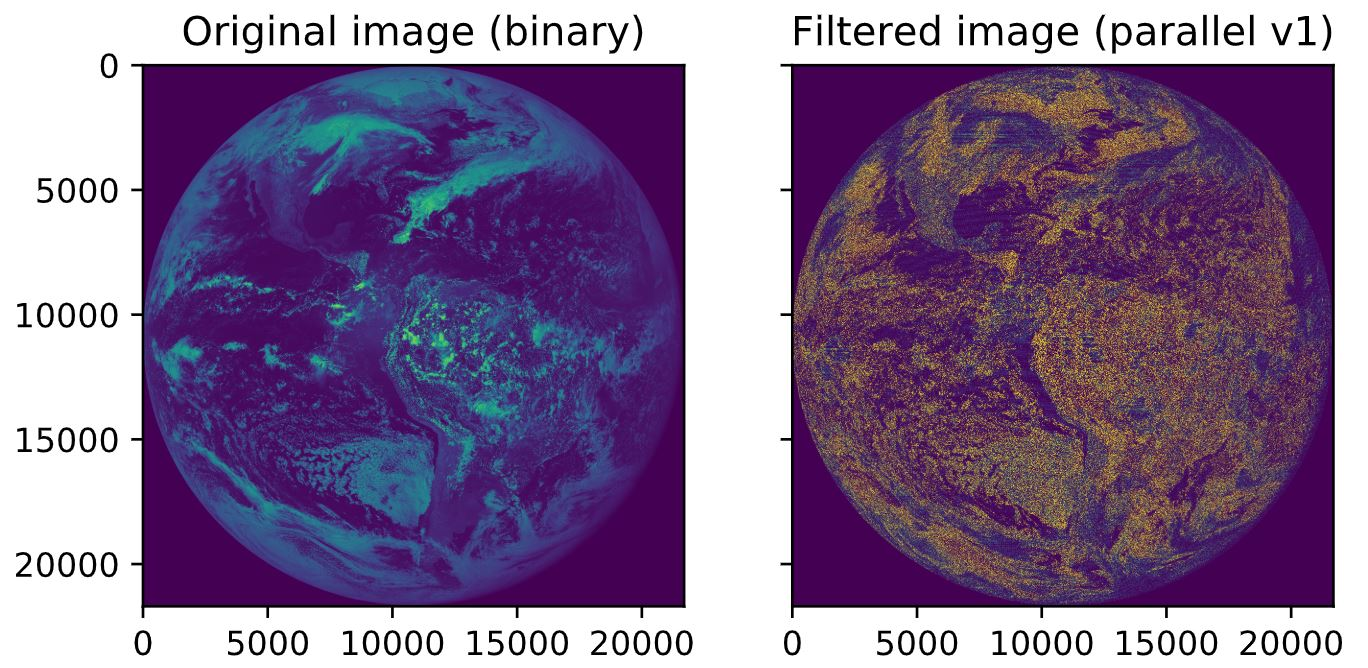
\includegraphics[width=0.9\textwidth]{figures/parallel1_1.jpg}
       \centering
       \caption{\textbf{\textcolor{Orange}{Imagenes, pero obtenidas de la explotación del paralelismo en la operación}}}
    \end{figure}
    
   \begin{figure}[H]
    \centering
      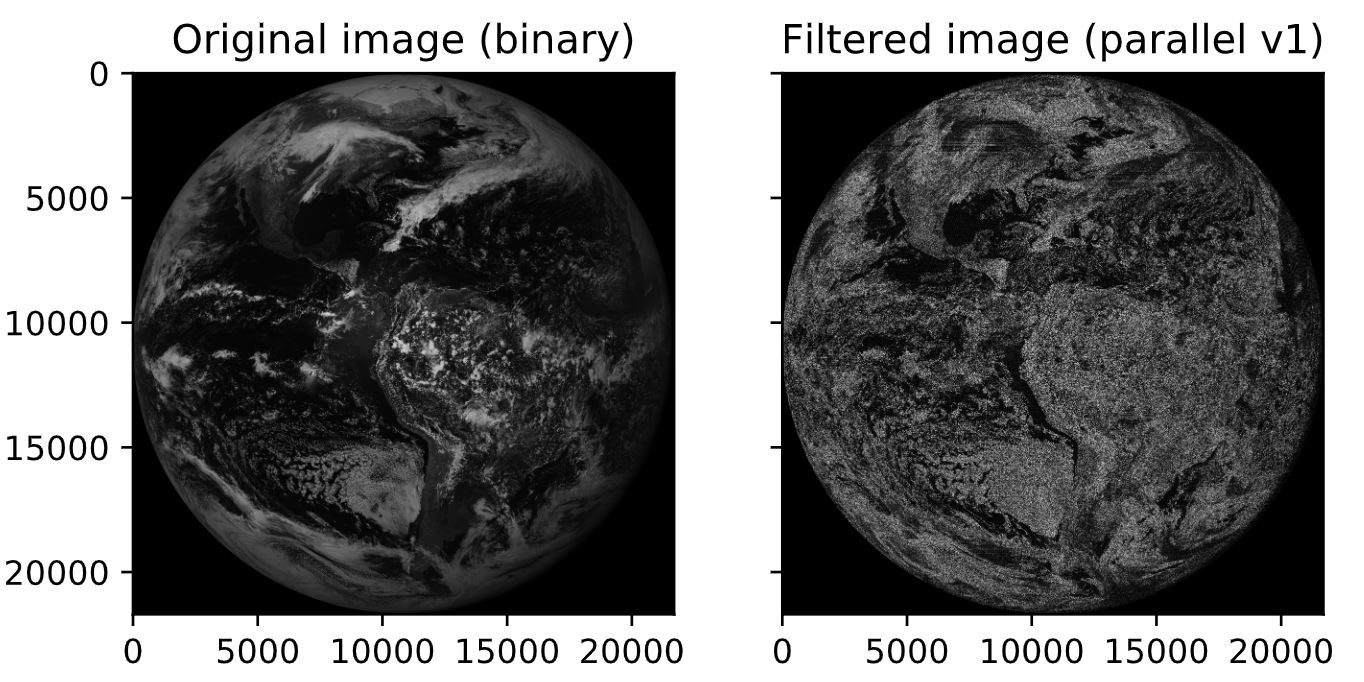
\includegraphics[width=0.9\textwidth]{figures/parallel1_2.jpg}
       \centering
       \caption{\textbf{\textcolor{Orange}{Imagenes, pero obtenidas de la explotación del paralelismo en la operación (escala de grises)}}}
    \end{figure}
    
    Recordando que se tratan de archivos binarios, veamos lo que obtenemos del segundo metodo de convolucion paralela, donde la salida se almaceno en un archivo \textit{.nc}:
  \begin{figure}[H]
    \centering
      \includegraphics[width=0.75\textwidth]{figures/outputpar_omp_for.png}
       \centering
       \caption{\textbf{\textcolor{Orange}{Imagen filtrada y ploteada desde archivo .nc (convolucion paralela v2)}}}
    \end{figure}
    

\subsection{Análisis de tiempo de ejecución}
Al principio de la seccion se anexaron las prestaciones del procesador de la maquina local \textit{intel i7-7700hq 2.80ghz}. El mismo consta de 4 nucleos fisicos, y 2 thread por nucleo. Para 50 corridas variando el numero de hilos (2, 4, 8, 12, 16, 20, se obtuvieron los
siguientes resultados:\\

  \begin{figure}[H]
    \centering
      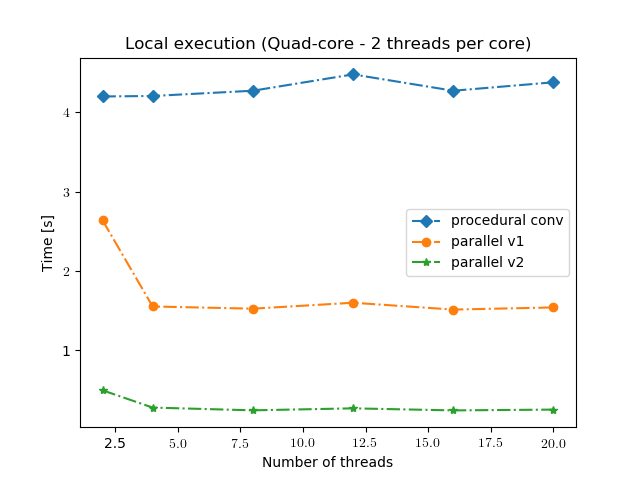
\includegraphics[width=0.69\textwidth]{figures/time_it.png}
       \centering
       \caption{\textbf{\textcolor{Orange}{Ejecución de 50 corridas del programa para cada numero de hilos instanciados}}}
    \end{figure}   

En cuanto al cluster (Xeon Gold 6130 , de 16 cores y 32 threads), se obtuvieron las siguientes curvas:\\
  \begin{figure}[H]
    \centering
      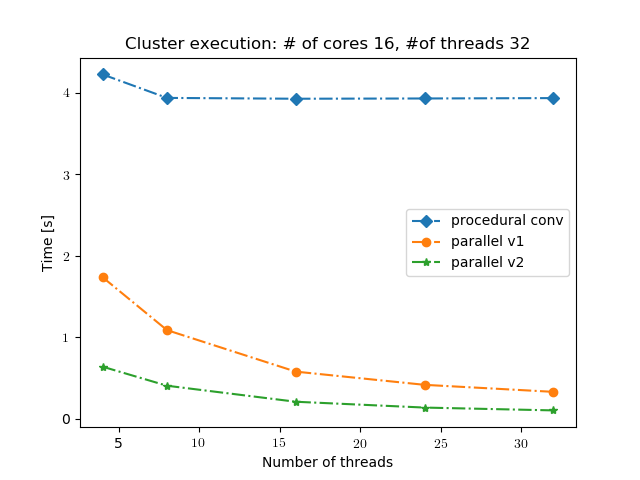
\includegraphics[width=0.75\textwidth]{figures/time_cluster.png}
       \centering
       \caption{\textbf{\textcolor{Orange}{Ejecución de 50 corridas en el cluster del programa para cada numero de hilos instanciados}}}
    \end{figure}   
    
 El tiempo en el eje $y$ es el tiempo promedio de las 50 ejecuciones por cada numero de threads instanciados. Se obtuvieron métricas temporales con la función mencionada, y se las almaceno en archivos. Dichos archivos luego, se leyeron efectuando un promedio de los 50 valores para cada tipo de convolución, por cada nivel de paralelismo (o cantidad de threads instanciados). Con esa recopilación de datos, se confeccionaron los gráficos anteriores.\\
 
 En la ejecución local se ve como a partir de que se supera el numero máximo dadas sus prestaciones, directamente se estanca el tiempo, o mejor dicho, no hay mejora, oscila.\\
 
A nivel tiempo no parece una desventaja drástica, pero cabe destacar que a nivel recursos dichos threads son instanciados y alternados en ejecución, por ende que la ejecución torna en si a ser deficiente. \\
 
 En cuanto al cluster, se ve la notoria diferencia en el promedio de tiempo de las 50 ejecuciones en las dos versiones paralelas, donde se llega a un tiempo casi un 45\% mas rápido que en la ejecución en la maquina local. \\
 

\section{Conclusiones}

Se puede ver que los resultados obtenidos en la computadora local son superados por los obtenidos del cluster. Esto se debe a las prestaciones de su procesador. \\

A su vez, paralelizar el problema planteado con OpenMP incrementa la performance del programa. Esto es por la paralelismo inherente de este tipo de operación, que si bien en la computadora local se llega a un mínimo rondando los 6 u 8 threads, en el cluster se ve claramente dicha disminucion notoria, llegando a un tiempo de 100[ms] en filtrar la imagen por completo. \\




\end{document}